\chapter{METHODOLOGY}

\section{System Block Diagram}
The system consists of three main stages: analog signal conditioning, digital processing for transient detection, and bone conduction output.
\begin{figure}[H]
    \centering
    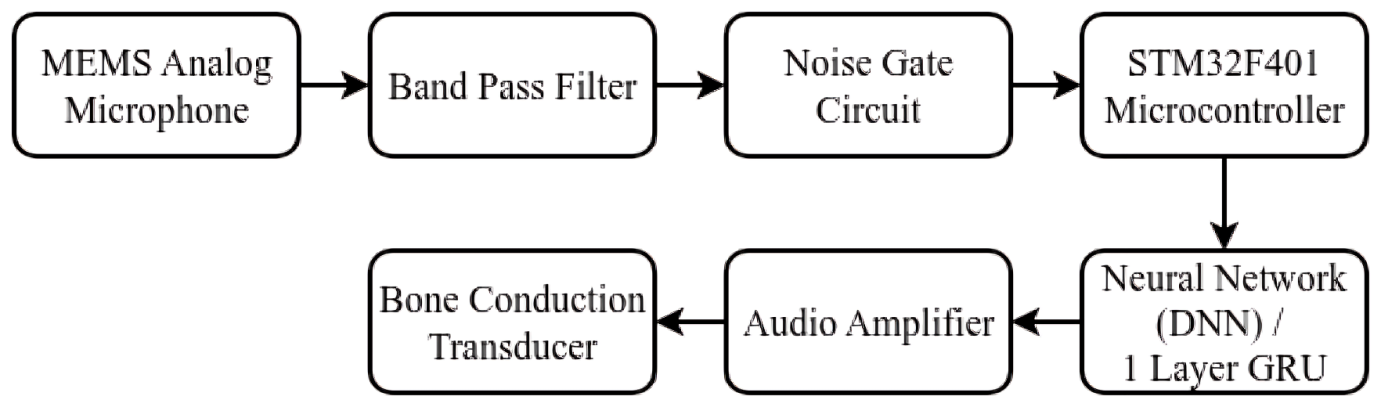
\includegraphics[width=1\linewidth]{src/images/blockDiagram.png}
    \caption{Block Diagram of the Proposed System}
    \label{fig:block_diagram}
\end{figure}

\section{Description of Working Principle}
Ambient sound is captured by an analog MEMS microphone. The signal passes through an active band-pass filter (300 Hz - 3.4 kHz) built with LM324 op-amps, which removes low-frequency rumble and high-frequency hiss. A noise gate (diode-capacitor peak detector + transistor) silences the output when the signal falls below a threshold, eliminating low-level static. The filtered analog signal is sampled by the STM32F401 ADC at 16 kHz. A tiny DNN running on the STM32 detects transient impulsive noises (door slam, footstep). If a transient is detected, the MCU pulls a control line low for 50 ms, momentarily muting the output via a transistor limiter. The signal is then amplified by an LM386 power amplifier and drives a bone conduction actuator pressed against the user's mastoid bone.

\section{Hardware Implementation}
\subsection{Microphone and Pre-amplification}
Component: Analog MEMS microphone (e.g., ADMP401, or salvaged equivalent).
Circuit: Non-inverting amplifier using LM324 with gain set to 20-50 dB to bring microphone output to line level.

\subsection{Active Band-Pass Filter}
Component: LM324 or NE5532 operational amplifiers, resistors, capacitors.

\subsection{Noise Gate}
Components: 1N4148 diode, electrolytic capacitor (10 \gls{symb:mu}F), BC547 transistor, resistors.
Operation: The diode-capacitor network rectifies and smooths the audio signal; the transistor switches off the audio path when the rectified voltage drops below a threshold set by a trimpot.

\subsection{Microcontroller and Transient Limiter}
Component: STM32F401 “Blue Pill” board, NPN transistor (BC547), resistor.
Connection: Filtered audio is fed to an ADC pin (PA0). A digital output pin (PA1) drives the base of the transistor placed in series with the audio signal. When the ML model detects a transient, the output pin goes high for 50 ms, shorting the audio to ground.

\subsection{Audio Power Amplifier and Bone Conduction Actuator}
Components: LM386 IC, 10 k$\omega$ potentiometer (volume control), 220 $\mu$F capacitor (output coupling), bone conduction actuator (e.g., generic 4$\omega$ 1-2W vibrator).
Circuit: Standard LM386 non-inverting amplifier (gain = 200) with the actuator connected via the coupling capacitor.

\subsection{Power Supply}
Components: 3.7V Li-ion battery (1000 mAh), TP4056 charger module or self-designed BMS.
Distribution: 3.7V directly powers the LM386 (works down to 4V). A 3.3V LDO (AM1117) on the STM32 board derives 3.3V for the MCU and op-amps.

\section{Software Implementation}
\subsection{Firmware on STM32F401}
ADC Configuration: 12-bit, continuous conversion mode, sampling rate 16 kHz using a timer trigger.
Buffering: Circular buffer of 40 samples (2.5 ms of audio).
TinyML Model: Pre-trained quantized int8 DNN with architecture: input layer (40), hidden dense layers (16, 16, 16, ReLU), output layer (1, sigmoid). Model size <20 KB flash, <5 KB RAM.
Inference: Every time the buffer is filled, call the STM32Cube.AI generated run\_inference() function. The output is a probability of a transient event.
Muting Logic: If probability > 0.8, set mute\_pin HIGH; start a non-blocking 50 ms timer; after timer expires, set pin LOW.

\subsection{Training the TinyML Model}
Dataset: Collected by recording 30 minutes of speech in background noise (fan, traffic) and 100 transient events (door slam, hammer, footstep) through the same analog front end.
Preprocessing: Frame extraction (40 samples per frame, 50\% overlap). Label frames: speech = 0, transient = 1.
Model Training: TensorFlow 2.x, Dense layers with ReLU, sigmoid output. Binary crossentropy loss, Adam optimizer, 20 epochs.
Quantization and Export: Convert to TensorFlow Lite (int8 quantization) then use STM32Cube.AI to generate C code.

\subsection{Integration}
Generated C model files are included in the STM32CubeIDE project.
Main loop: ADC DMA fills buffer → inference → update mute pin.

\section{Instrumentation Tools}
Hardware: Oscilloscope (for filter tuning), multimeter, soldering station, breadboard.
Software: STM32CubeIDE, STM32Cube.AI, TensorFlow 2.x, Audacity (for dataset recording).
